%
\subsection{Linear flat-plate cascade}
\label{LINSUB.subsec}
%
\begin{figure}
  \begin{center}
  \begin{tabular}{cc}
    \subfigure[Geometry]
      {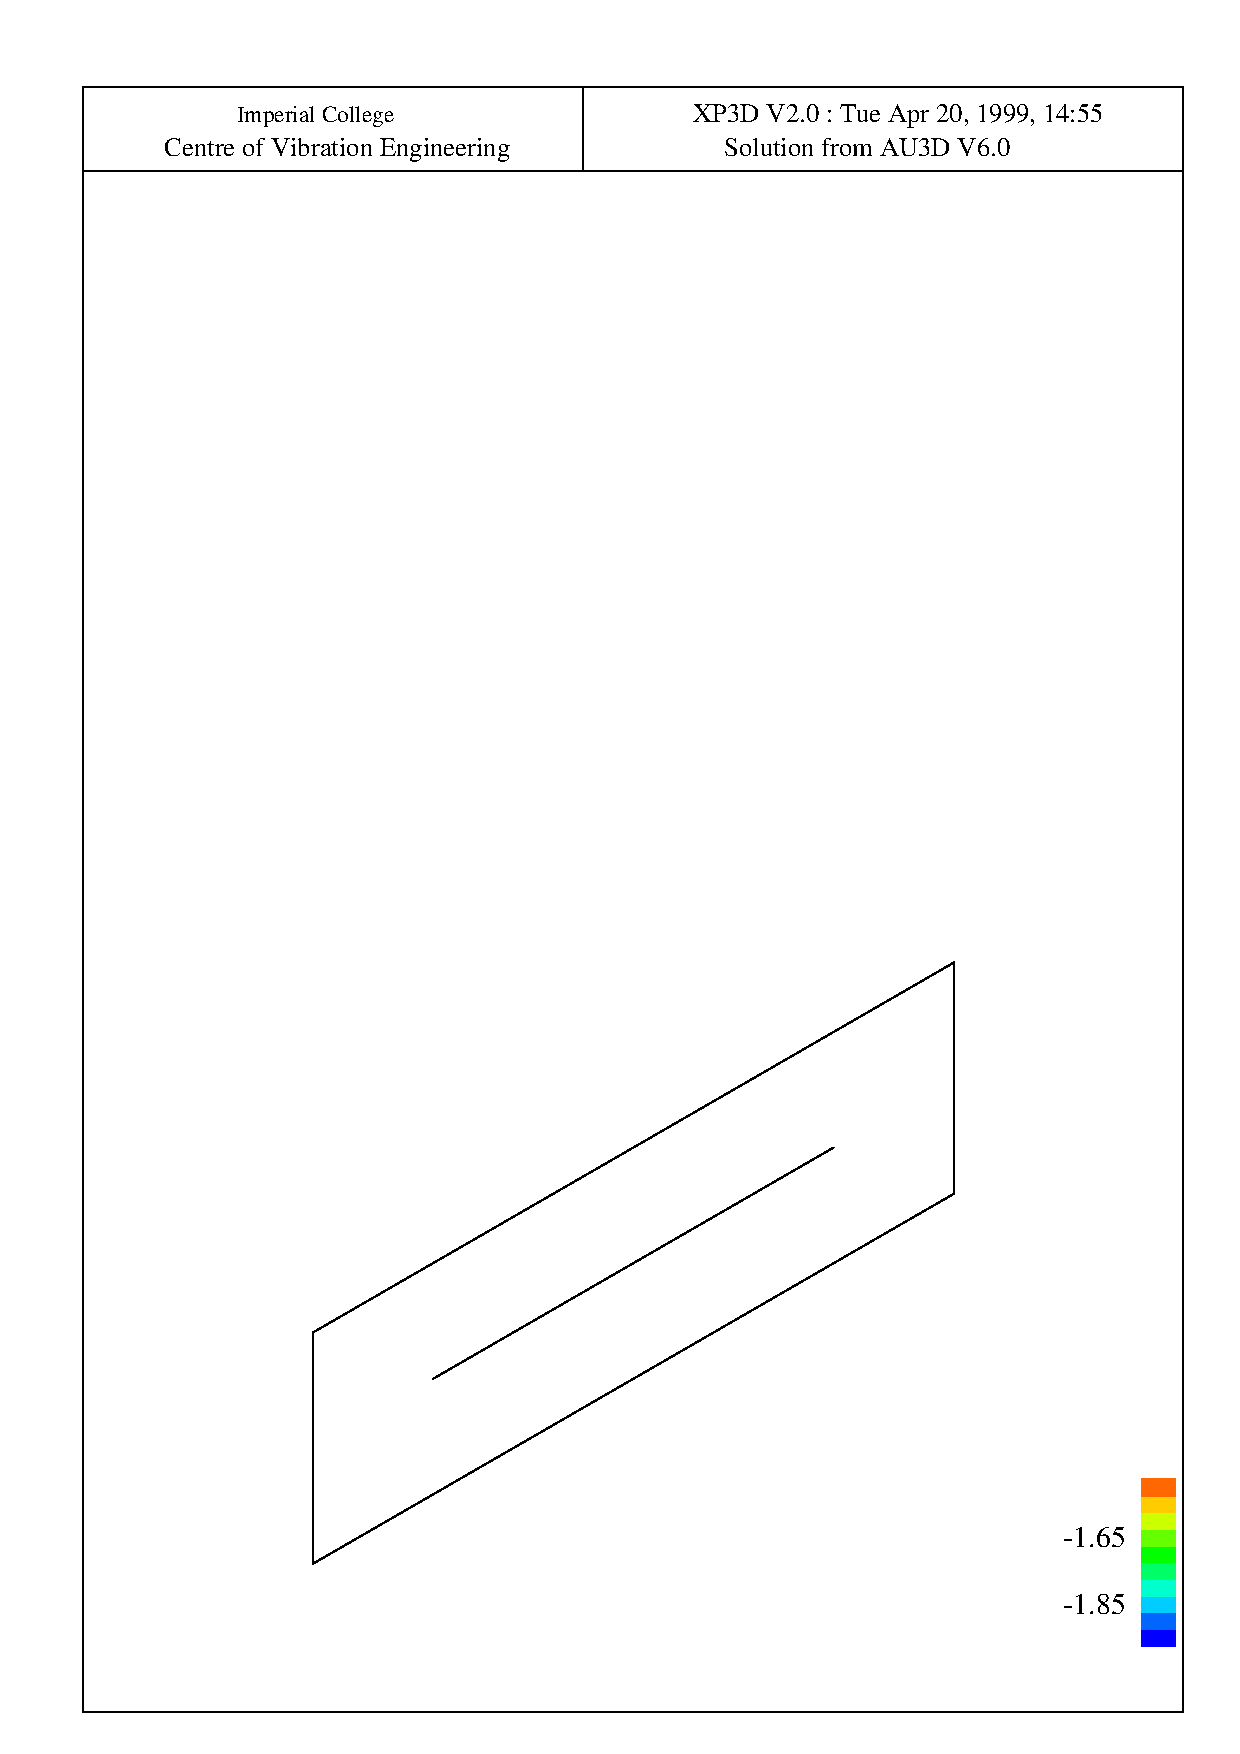
\includegraphics[width=70mm,clip=t]{CHAP_LINEAR/FIGURE/lins_geom.pdf}
       \hspace{0mm}} &
    \subfigure[Computational domain (2,232 points)]
      {\hspace{0mm}
        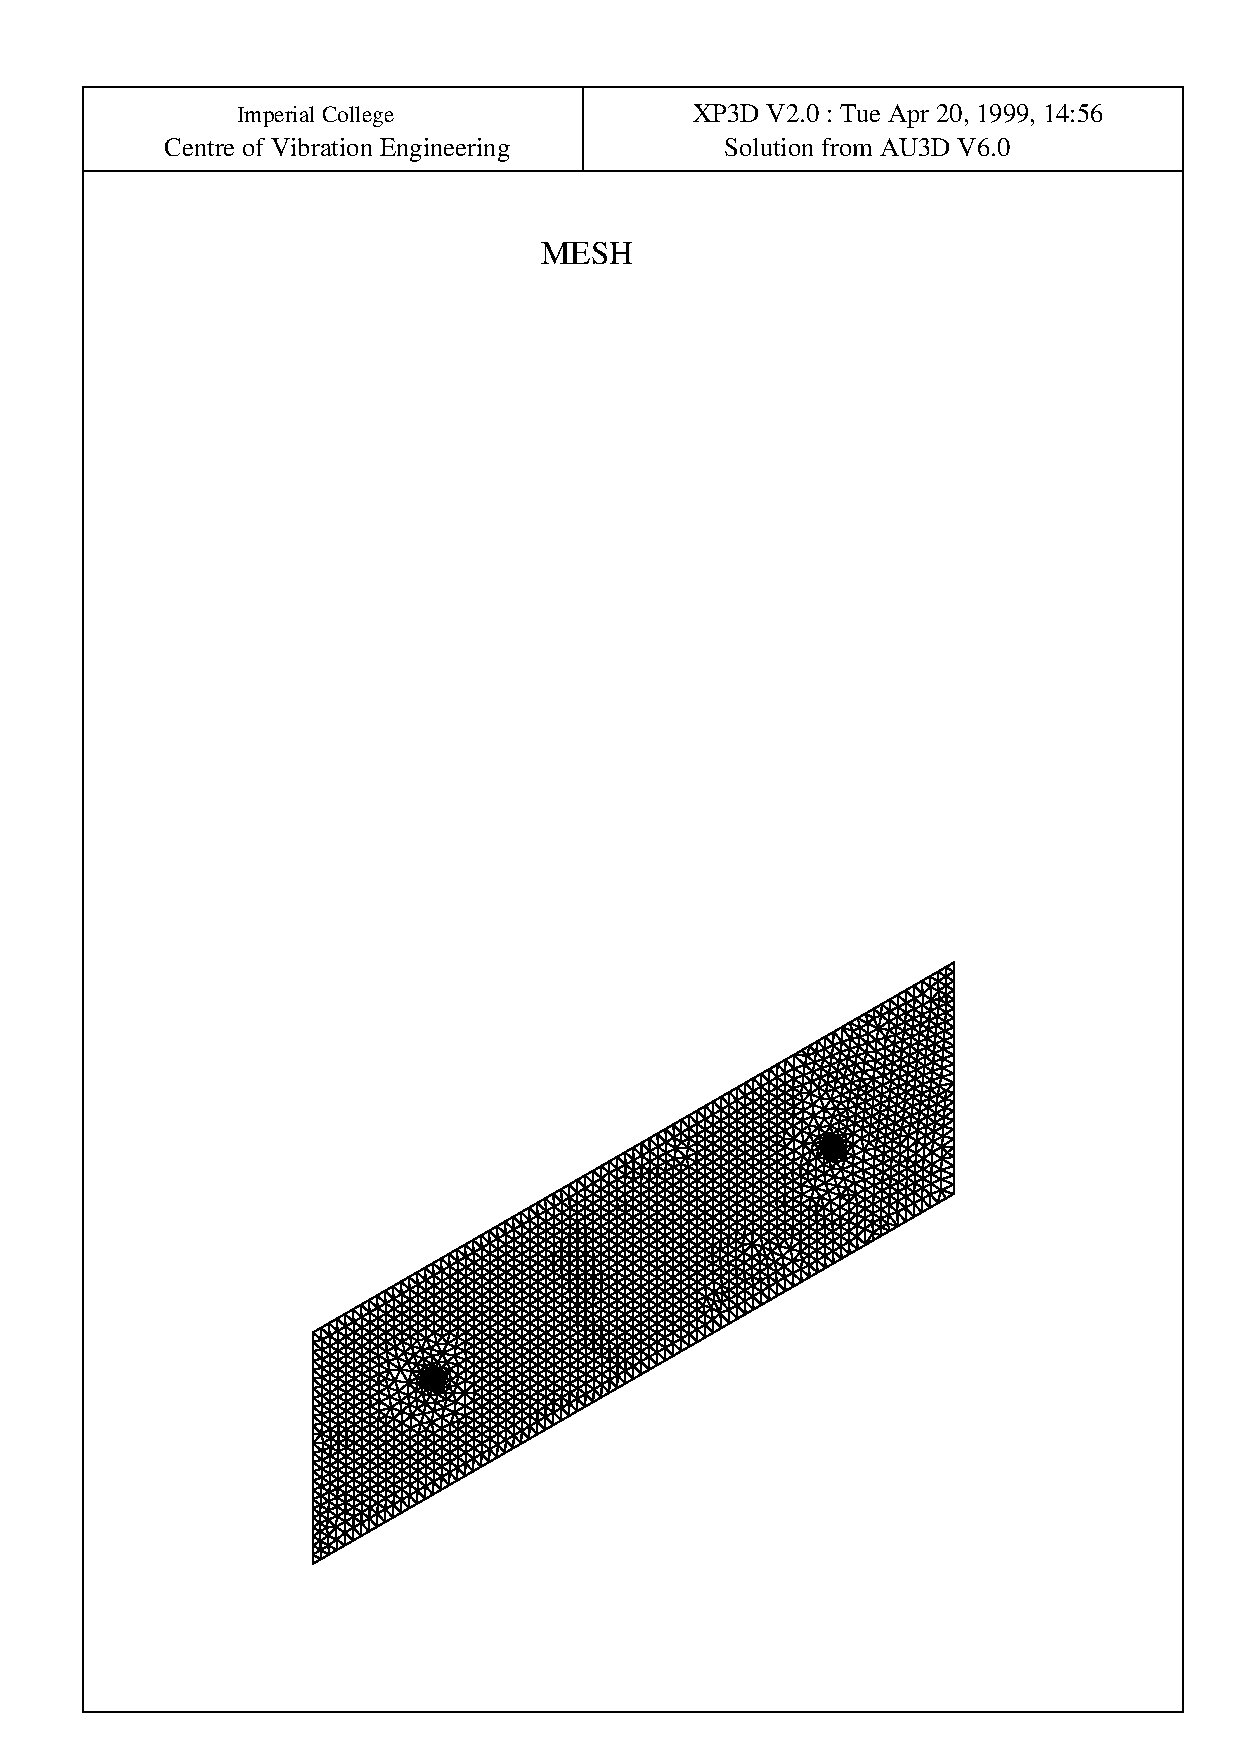
\includegraphics[width=70mm,clip=t]{CHAP_LINEAR/FIGURE/lins_mesh.pdf}}
   \end{tabular}
 \end{center}
 \vspace{-8mm}
 \caption{Flat plate cascade. Geometry and computational domain}
 \label{linsub_geom_mesh.fig}
\end{figure}
%
%
\begin{figure}
  \begin{center}
  \begin{tabular}{c}
    \subfigure[Real part]
       {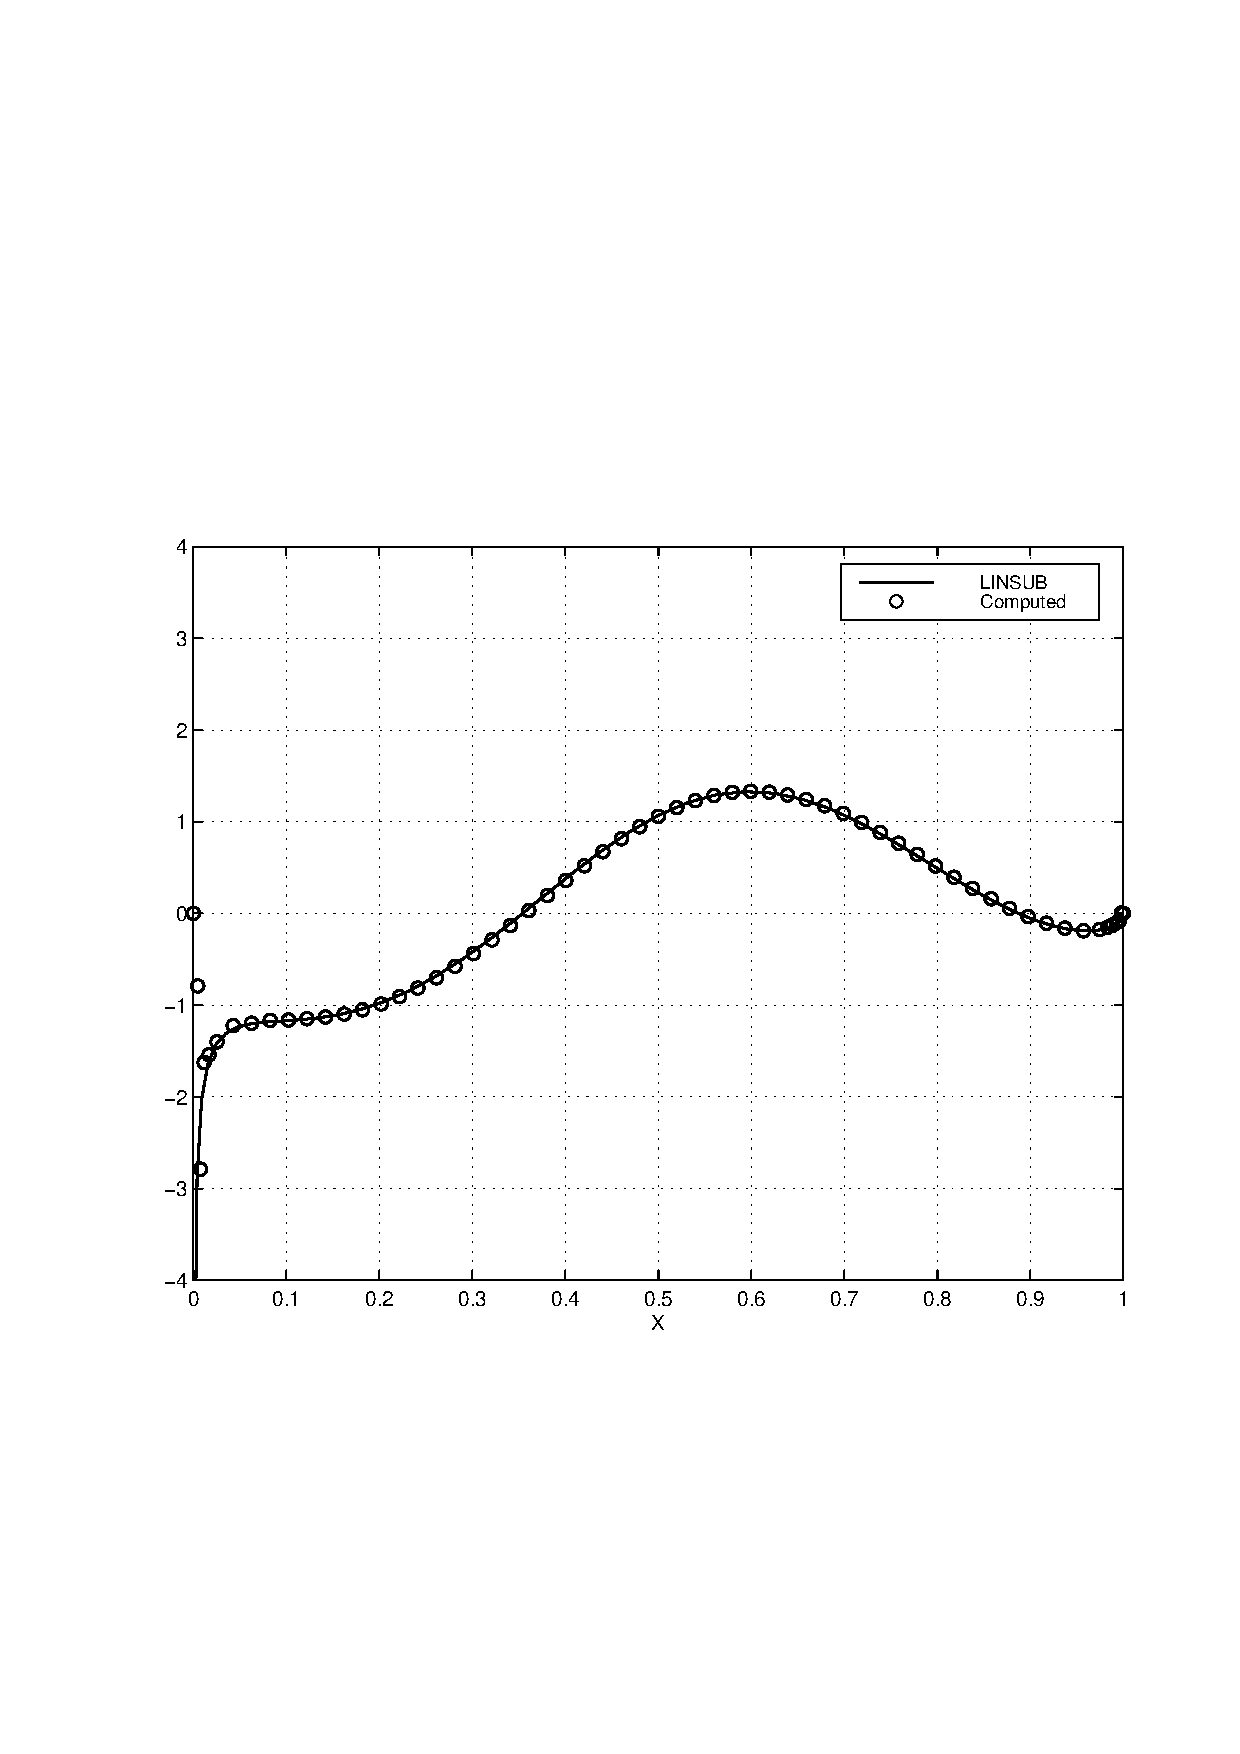
\includegraphics[width=110mm,clip=t]{CHAP_LINEAR/FIGURE/lins_wake1.pdf}
       \hspace{0mm}} \\
    \subfigure[Imaginary part]
      {\hspace{0mm}
        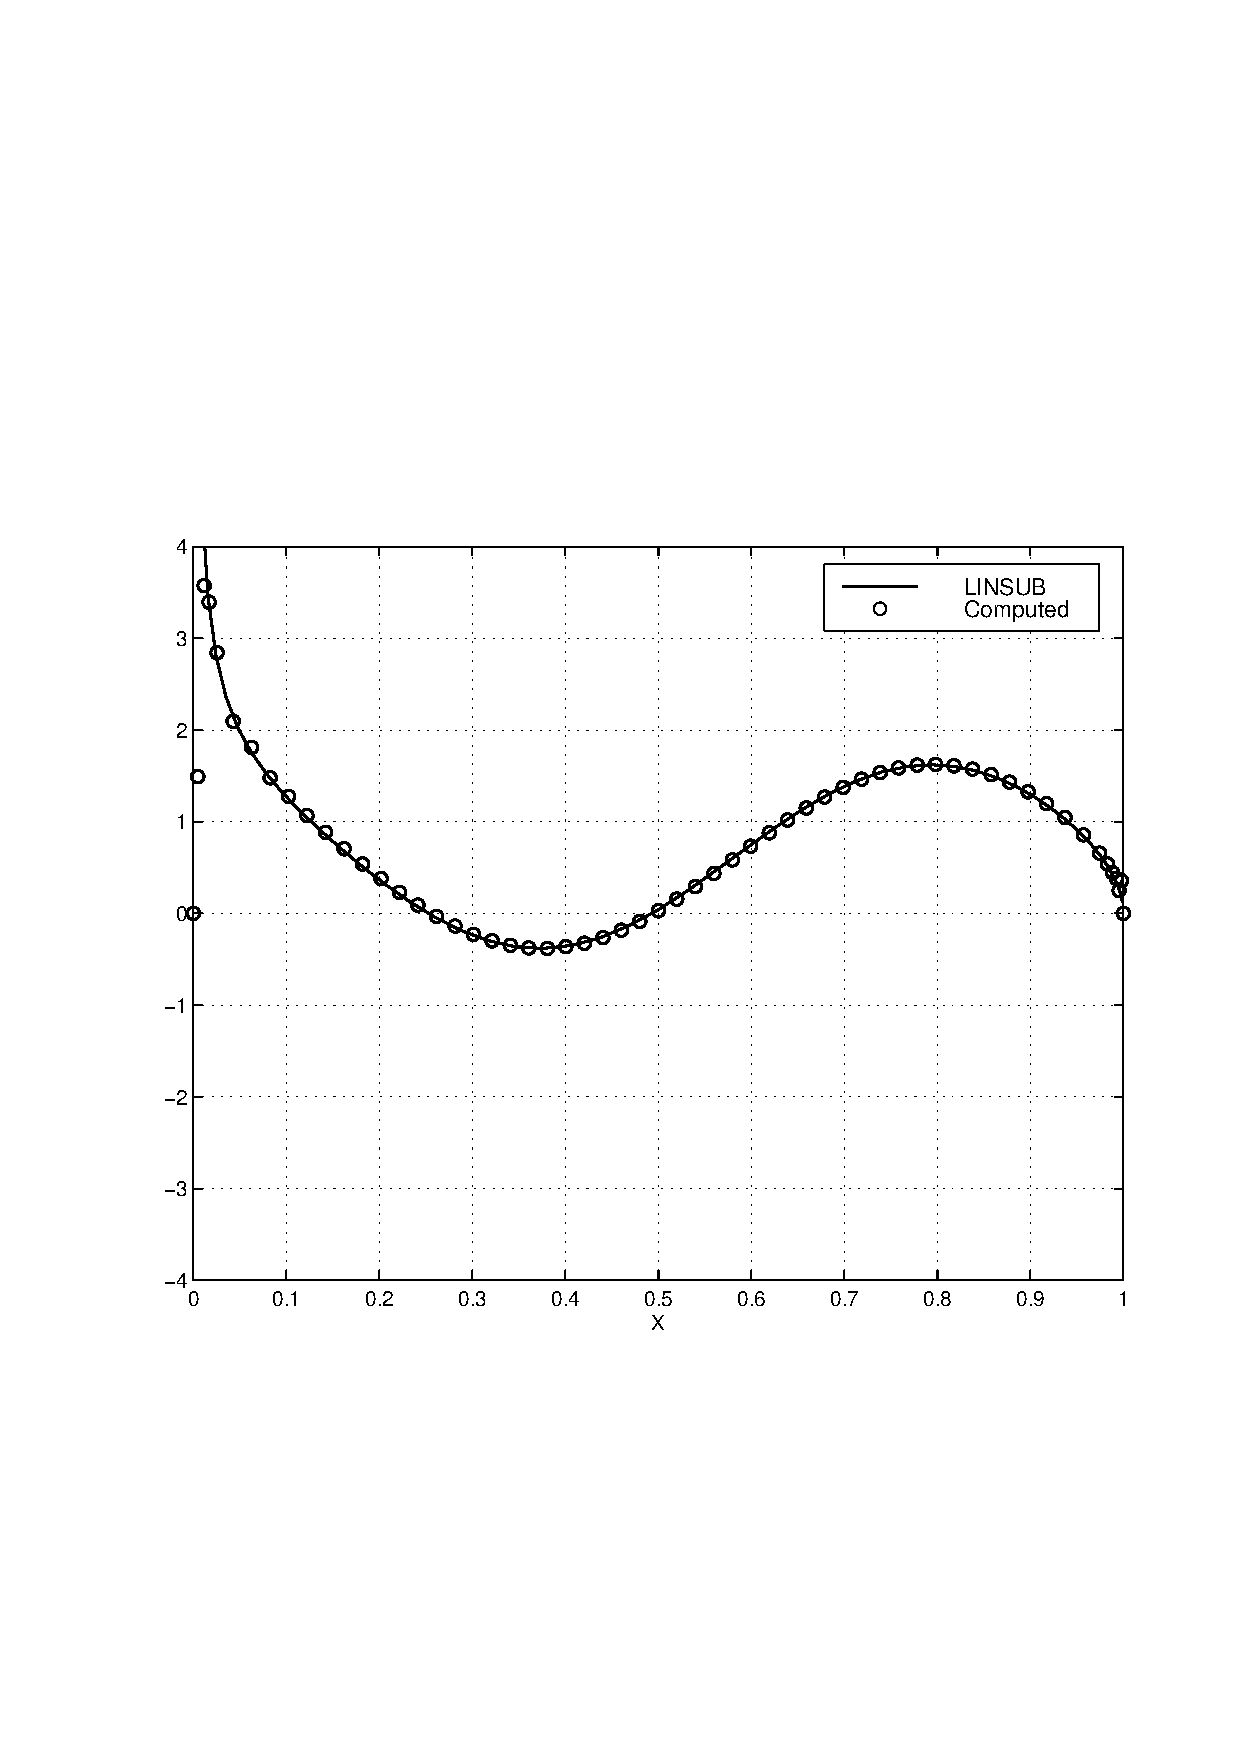
\includegraphics[width=110mm,clip=t]{CHAP_LINEAR/FIGURE/lins_wake2.pdf}}
   \end{tabular}
 \end{center}
 \vspace{-8mm}
 \caption{LINSUB test case. Pressure jump on flat plate due to wake/rotor interaction
          ($\omega = \pi$, $\phi = -90\se{o}$)}
 \label{linsub_wake.fig}
\end{figure}
%
\begin{figure}
  \begin{center}
  \begin{tabular}{c}
    \subfigure[Real part]
       {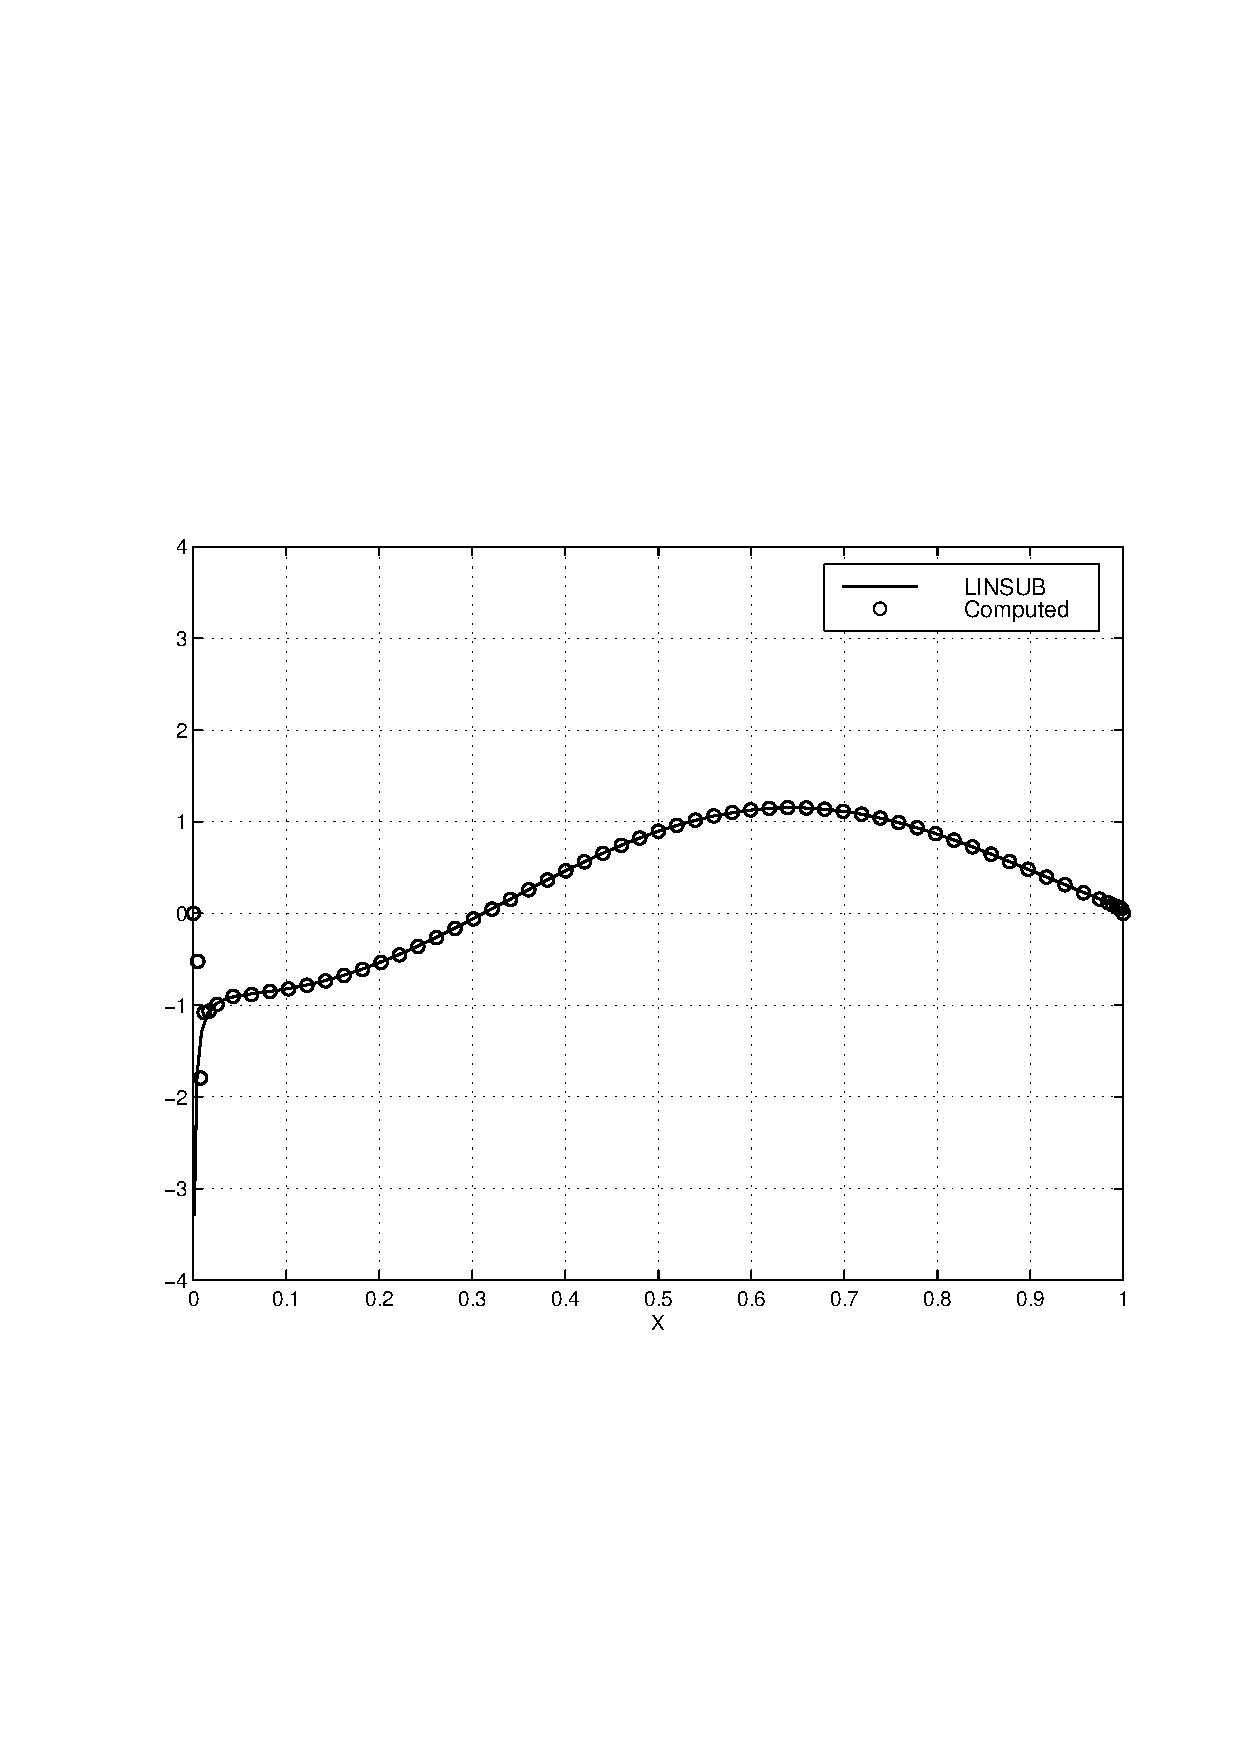
\includegraphics[width=110mm,clip=t]{CHAP_LINEAR/FIGURE/lins_pres1.pdf}
       \hspace{0mm}} \\
    \subfigure[Imaginary part]
      {\hspace{0mm}
        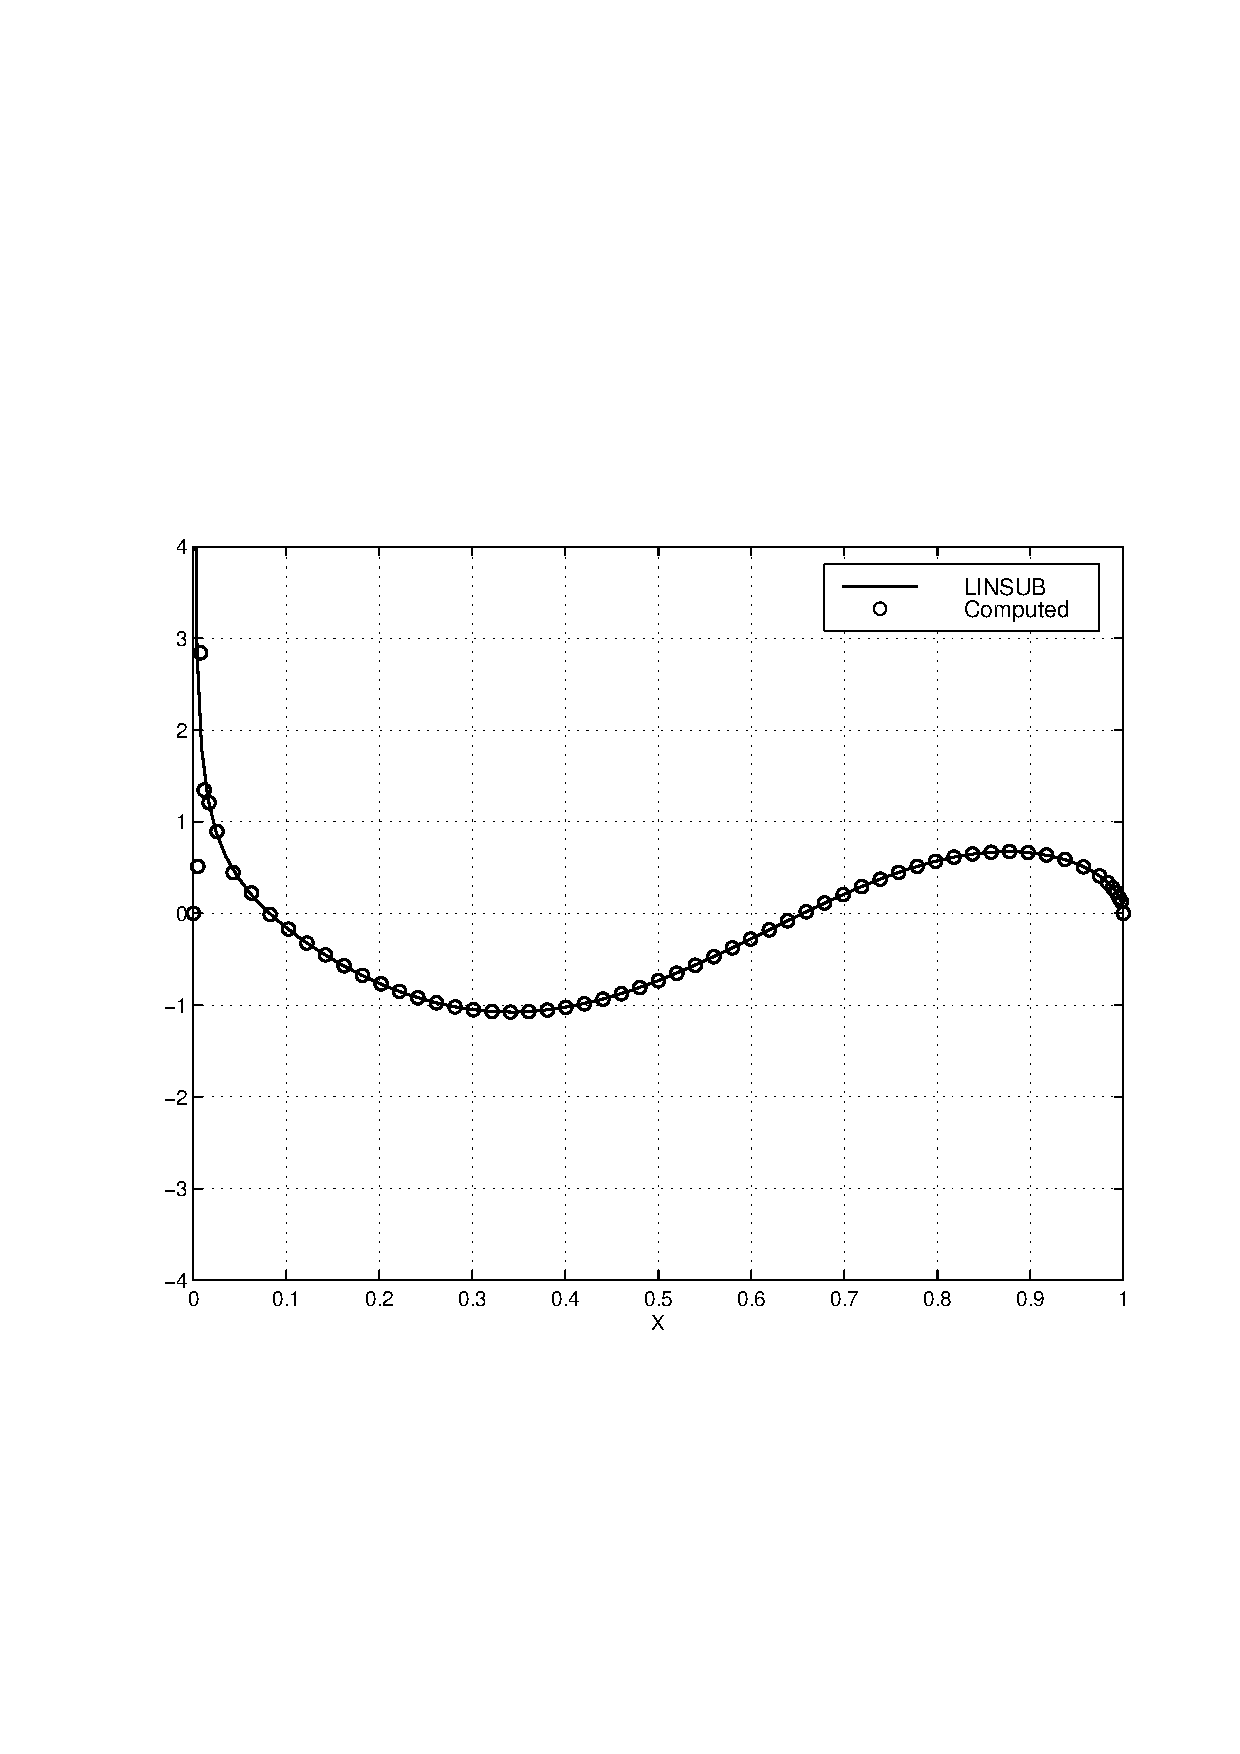
\includegraphics[width=110mm,clip=t]{CHAP_LINEAR/FIGURE/lins_pres2.pdf}}
   \end{tabular}
 \end{center}
 \vspace{-8mm}
 \caption{LINSUB test case. Pressure jump on flat plate due to upstream acoustic wave
          ($\omega = 2$, $\phi = 0\se{o}$)}
 \label{linsub_pres.fig}
\end{figure}
%
\begin{figure}
  \begin{center}
  \begin{tabular}{c}
    \subfigure[Real part]
       {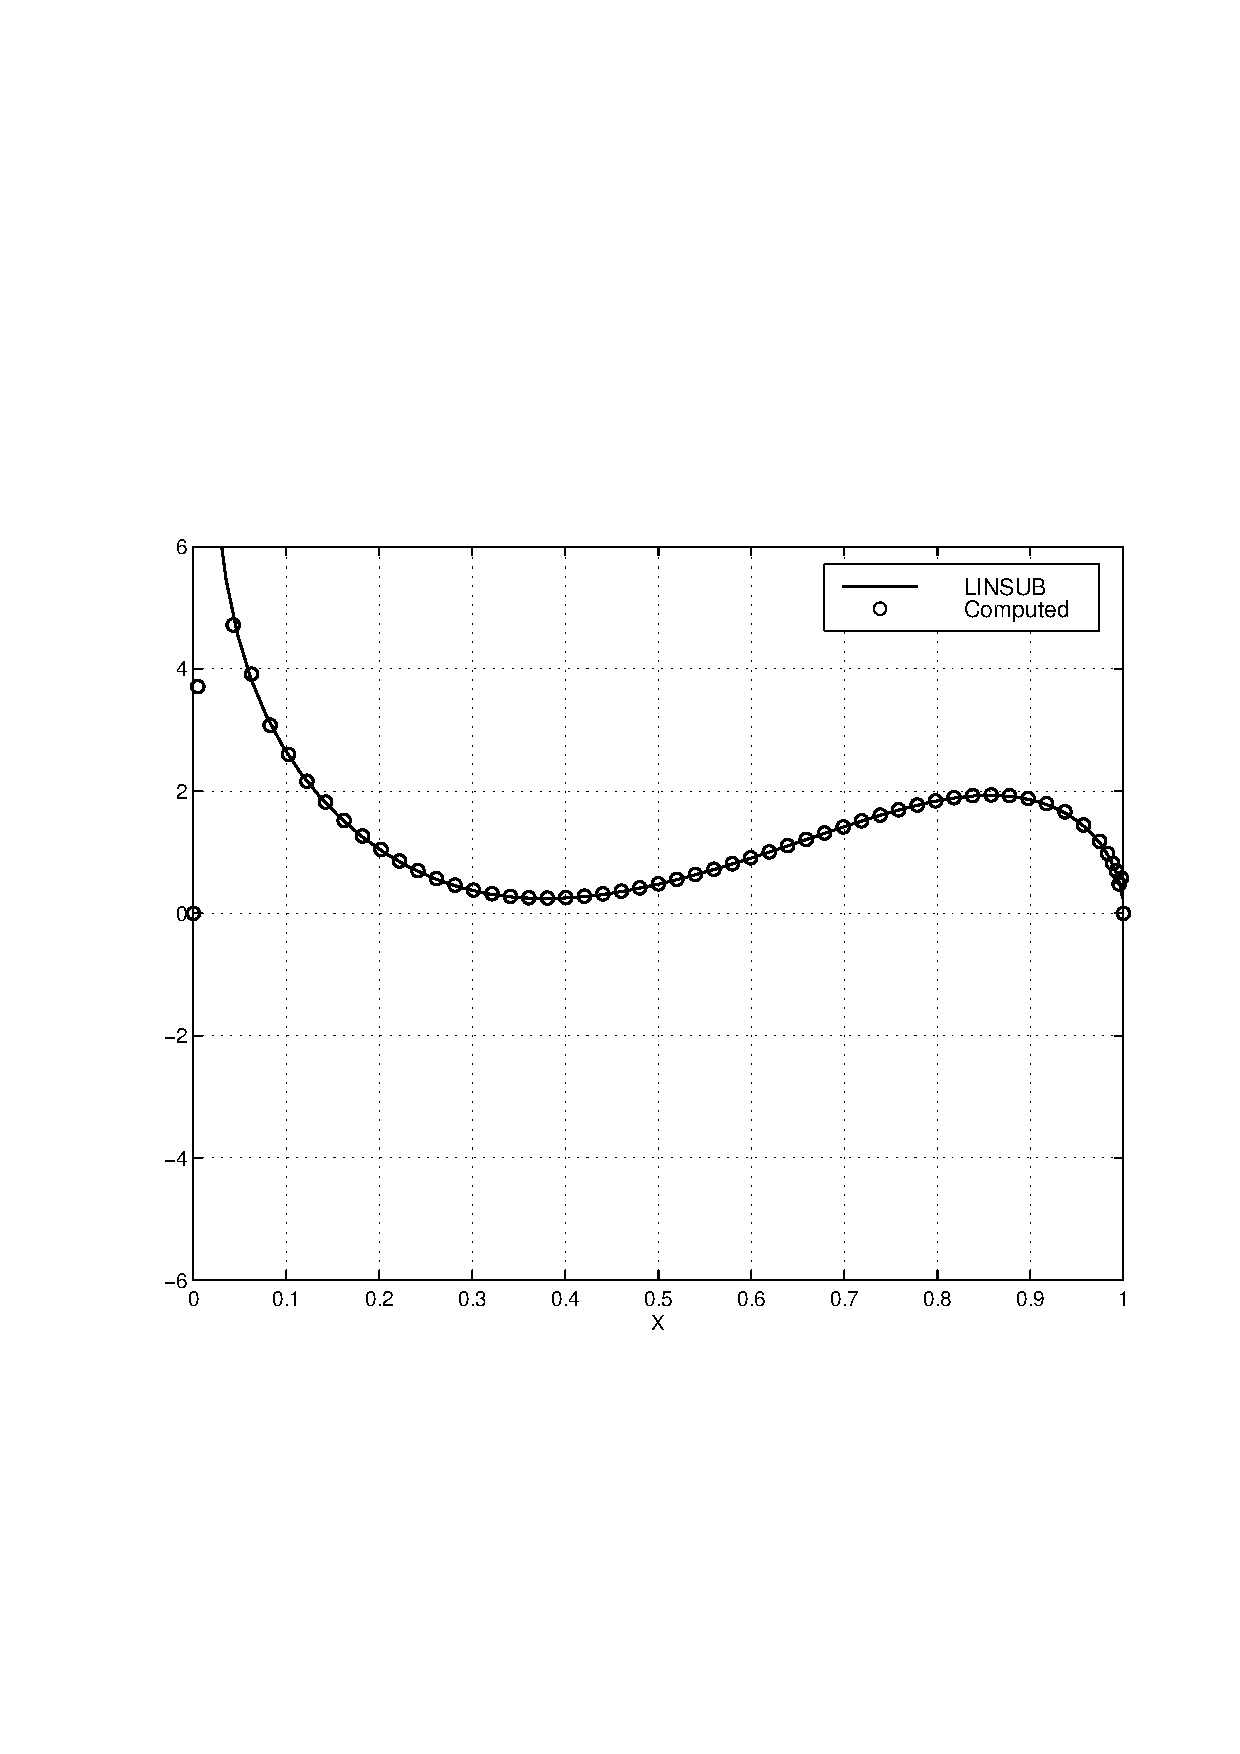
\includegraphics[width=110mm,clip=t]{CHAP_LINEAR/FIGURE/lins_bend1.pdf}
       \hspace{0mm}} \\
    \subfigure[Imaginary part]
      {\hspace{0mm}
        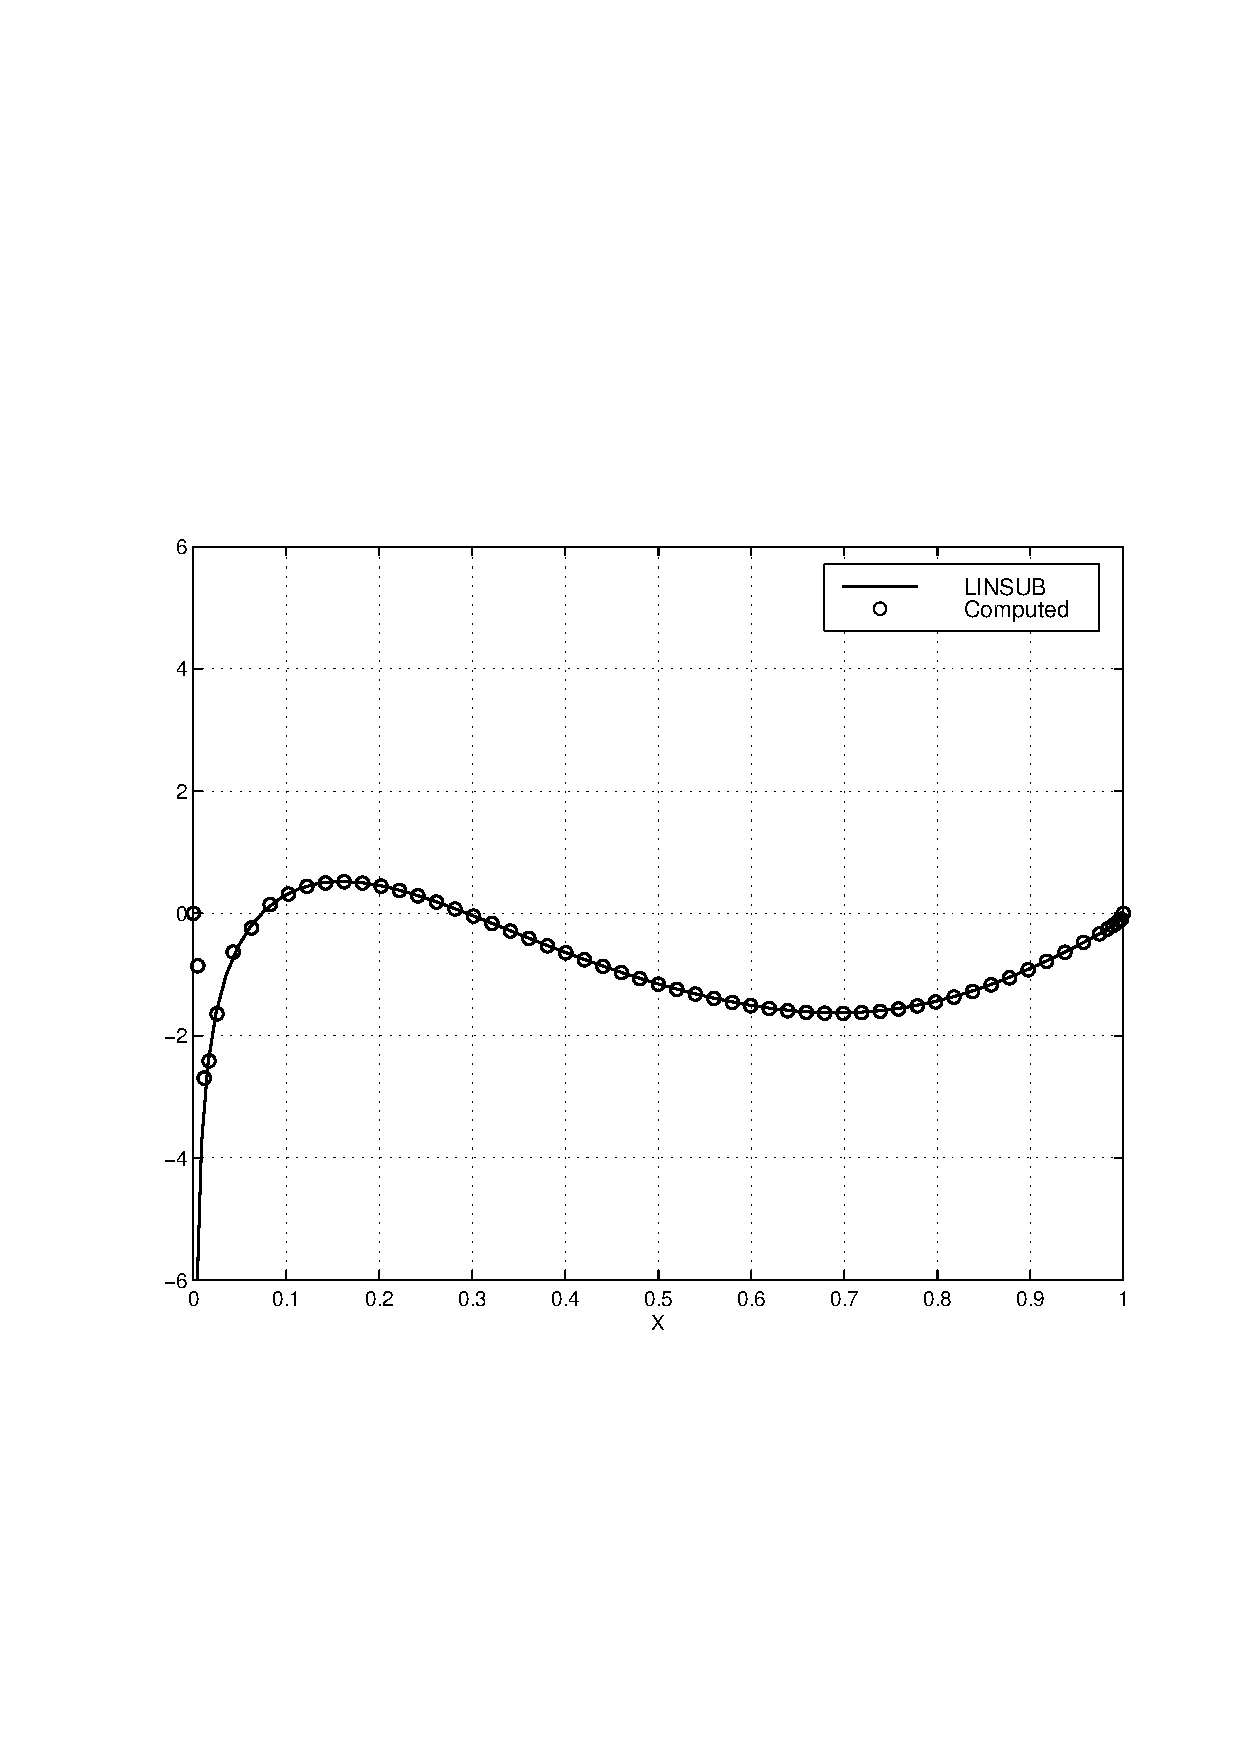
\includegraphics[width=110mm,clip=t]{CHAP_LINEAR/FIGURE/lins_bend2.pdf}}
   \end{tabular}
 \end{center}
 \vspace{-8mm}
 \caption{LINSUB test case. Pressure jump on flat plate due to bending oscillation
          ($\omega = 2$, $\phi = 90\se{o}$)}
 \label{linsub_bend.fig}
\end{figure}
%
%
 Small-amplitude perturbations of a uniform, inviscid steady-state flow past an
 unloaded flat-plate cascade are studied first.  Such cascades can  be used for a
 variety of applications: wake/blade interaction, potential/blade interaction, aeroelasticity
 studies by including the blade's bending and torsional motion. The main aerodynamic
 parameters are the Mach number, reduced frequency, pitch-to-chord ratio, stagger
 angle and the interblade phase angle.

 Three different disturbances were studied for  a pitch-to-chord ratio of 0.5,
 a stagger angle of $30\se{o}$ and a mean-flow Mach number of 0.7.
 For all three cases, the results were checked against the benchmark LINSUB code
 by plotting the real and imaginary parts of the (complex) unsteady pressure difference across
 the plate.  The geometry and the computational domain  are
 shown in Fig. \ref{linsub_geom_mesh.fig}. The mesh has high resolution around the
 trailing and leading edges in order to handle the singularities which occur
 in these regions.

 The first disturbance simulates a wake/blade interaction, an incoming
 sinusoidal wake with a reduced frequency of $\pi$ being specified at the inflow boundary.
 The  interblade phase angle is $-90\se{o}$. Fig. \ref{linsub_wake.fig}
 shows  excellent agreement between the present method and the benchmark program LINSUB.
 The second disturbance simulates potential/blade interaction,  an
 incoming pressure wave with a reduced frequency of $2.0$ being specified
 at the outflow boundary. The interblade phase angle is $0\se{o}$.
 Fig. \ref{linsub_pres.fig} shows excellent agreement between the present method and the
 benchmark program LINSUB.
 The last disturbance  studied is for a bending motion with a reduced frequency of
 $2.0$ and an interblade phase angle of $90\se{o}$. Once again, excellent agreement
 is observed from Fig. \ref{linsub_bend.fig}.
%
